\documentclass{article}
\usepackage[utf8]{inputenc}
\usepackage[margin=1.5in]{geometry}
\usepackage{amsmath}
\usepackage{amssymb}
\usepackage{xcolor}
\usepackage{hyperref}
\usepackage{slashed}
\usepackage{graphicx,caption}
\usepackage{subcaption}
\usepackage{tikz}
\usepackage{esint}
\usepackage{tikz-feynman}
\usepackage{lipsum}
\usepackage{placeins}
\usepackage{array}
\hypersetup{
        bookmarksnumbered,
        unicode,                        % use with \texorpdfstring
        colorlinks,                     % avoid stupid boxes
        citecolor=[rgb]{.9,0,.5},       % \cite
        urlcolor=[rgb]{0,0,1},  % \href
        linkcolor=[rgb]{0,.7,0} % \ref , toc
        }

\usepackage[
    %backend=biber, 
    natbib=true,
    style=numeric,
    sorting=none
]{biblatex}

\usepackage{feynmp-auto}
%\usepackage{feynman}

\newcommand{\bref}[1]{(\ref{#1})}
\newcommand{\pd}{\partial}
\newcommand{\sh}{\textrm{\,sh}}
\newcommand{\ch}{\textrm{\,ch}}
\renewcommand{\th}{\textrm{\,th}}
\renewcommand{\Im}{\textrm{Im\,}}
\renewcommand{\Re}{\textrm{Re\,}}
\newcommand{\yp}[1]{{\color{purple} #1}}
\DeclareMathOperator*{\Res}{Res}
\title{Notes on `t Hooft's model}
\author{Yu-Ping Wang}
\date{\today}

\begin{document}
\maketitle
\tableofcontents


\section{2D QCD}
\paragraph{}The Lagrangian of two-dimensional QCD with $U(N)$ gauge group with $m$-flavors of Dirac fermions is
\[
	{\cal L} = \frac{1}{4}\textrm{tr}F_{\mu\nu}F^{\mu\nu} - q_{a}\left(i\slashed{D}-m_{a}\right)\overline{q}^{a}, \quad a = 1, \cdots m.
\]
We shall set up some basic notations.  $\slashed{D} = \gamma^{\nu}D_{\nu}$ is the Dirac derivatives, and
\[
	F_{\mu\nu} = \pd_{\mu}A_{\nu}-\pd_{\nu}A_{\mu} + g \left[A_{\mu}, A_{\nu}\right], \quad  D_{\mu}q^{a} = \pd_{\mu}q^{a} + g \overline{A}_{\mu}\cdot q^{a}.
\]
$\overline{A}_{\mu} = A_{\mu} - \frac{1}{N}I \textrm{tr}A_{\mu}$ is the traceless part of $A_{\mu}$.

Its more convenient to use the light-cone coordinate.
\[
	x_{\mu} = (x_{+}, x_{-}), \quad x_{\pm}  = \frac{1}{\sqrt{2}}\left( x_{0}\pm x_{1}\right).
\]
The momentum in light-cone coordinate is denote similarly as $p_{\pm}=\frac{1}{\sqrt{2}}\left( p_{0}\pm p_{1}\right)$, and the inner product is $a_{\mu}b^{\mu} = a_{+}b_{-} + a_{-}b_{+}$. This means that when raising/lowering the indices, the plus and minus sing needs to be exchanged.

In two-dimensons, we are allowed to choose a gauge of $A_{\mu}$ such that $A_{-} = A^{+}$ =0. We also list out the explicit values of the gamma matrices $\gamma_{\mu}$.

\[
	\gamma_{\mu} \rightarrow \gamma_{\pm}, \quad \gamma_{+} =
	\begin{pmatrix}
		0 & 1 \\
		0 & 0
	\end{pmatrix},\;
	\gamma_{-} =
	\begin{pmatrix}
		0 & 0 \\
		1 & 0
	\end{pmatrix}.
\]
In this gauge, the Lagrangian could be explicit written down
\[
	{\cal L} = -\frac{1}{2}\textrm{tr}\left(\pd_{-}A_{+}\right)^2 - q_{a}\left(i\gamma_{+}\pd_{-}+ i\gamma_{-}\pd_{+} + m_{a} +g\gamma_{-}\overline{A}_{+} \right)\overline{q}^{a}.
\]

The advantage of choosing the light-cone gauge is there are no direct interactions between the gluons. Making the Feynman diagrams much simpler.  Since $A_{\mu}$ is a $U(N)$ matrix, we could use the double line notation for the gluon propagators.

The Feynman rules are the following:
\begin{center}
	\begin{tabular}{m{0.3\textwidth} m{0.3\textwidth} m{0.3\textwidth}}
		\begin{tikzpicture}[baseline={([yshift=-1.5ex]i1.base)}]
			\begin{feynman}
				\vertex at (0, 1) (i1) ;
				\vertex at (0, 0.8) (i2) ;
				\vertex at (3 , 1) (i3);
				\vertex at (3, 0.8) (i4);
				\vertex at (1.5, 0.8) (a);
				\diagram*{
				(i1) -- [fermion] (i3),
				(i4) -- [fermion] (i2),
				};
			\end{feynman}
		\end{tikzpicture}  & \( -\frac{i}{k_{-}^2}\)                                                                     & Gluon propagator                                                        \\[1em]
		\begin{tikzpicture} [baseline={([yshift=-1.5ex]i1.base)}]
			\begin{feynman}
				\vertex at (0, 1) (i1) {\(i\)} ;
				\vertex at (3 , 1) (i3){\(j\)} ;
				\vertex at (1.5, 1) (a);
				\vertex at (1.5, 1.3)(b) {\(a\)};
				\diagram*{
				(i1) -- [fermion] (i3),
				};
			\end{feynman}
		\end{tikzpicture} & \( \frac{i}{\gamma_{+}p_{-} + \gamma_{-}p_{+} -m_{a} -i\epsilon}\)                          &                                                                          \\ [1em]
		                                                     & = \(i\frac{\gamma_{+}p_{-} + \gamma_{-}p_{+} + m_{a}}{2p_{+}p_{-} - m_{a}^2 - i\epsilon} \) & Fermion propagator                    \\[1em]
		\begin{tikzpicture}[baseline={([yshift=-5.5ex]i1.base)}]
			\begin{feynman}
				\vertex at (0, 0) (i1) ;
				\vertex at (0, 0.2) (i2) ;
				\vertex at (1.7 , 0) (a);
				\vertex at (1.7, 0.2) (b);
				\vertex at (2.5, 1.2) (i3) {\(i\)};
				\vertex at (2.5, -1) (i4)  {\(j\)};
				\diagram*{
				(i4) -- [fermion] (a) -- [fermion] (i1),
				(i2) -- [fermion] (b) -- [fermion] (i3),
				};
			\end{feynman}
		\end{tikzpicture}
		                                                     & \(  ig \gamma_{-} \)                                                                        & Gluon-quark interaction               \\[3em]
		\begin{tikzpicture}[baseline={([yshift=-5.5ex]i1.base)}]
			\begin{feynman}
				\vertex at (0, 0) (i1) ;
				\vertex at (0, 0.2) (i2) ;
				\vertex at (2.5, 1.2) (i3) {\(i\)};
				\vertex at (2.5, -1) (i4) {\(j\)};
				\vertex at (1.7 , 0)  (a);
				\vertex at (1.7, 0.2) (b);
				\vertex at (1.5 , 0)  (a1);
				\vertex at (1.5, 0.2) (b1);
				\diagram*{
				(i4) -- [fermion] (a) -- (b) -- [fermion] (i3),
				(i2) -- [fermion] (b1) --  (a1) -- [fermion] (i1),
				};
			\end{feynman}
		\end{tikzpicture}
		                                                     & \(-\frac{i}{N}g\gamma_{-}\)                                                                 & Higher order gluon-quark interaction.
	\end{tabular}
\end{center}

We are interested in the large-$N$ limit. By the standard argument form `t Hooft, the planar graphs with no fermion loops are leading order, and we shall only consider `t Hooft model with one fermions and drop the index $a$.

\subsection{Quark Propagators}
We shall first study the fermion propagators in the leading order of large-$N$ limit. As illustrated in figure \ref{fig1}, if we denote $i\Gamma(p)$ as the sum of all one-particle irreducible diagrams, the fermion propagator $S(p)$ is the sum of all series of $\Gamma(p)$.
\[
	iS(p) = i\Delta(p) + i\Delta(p) i\Gamma(p)i\Delta(p) + \cdots = -\frac{i}{\gamma_{+}p_{-}+ \gamma_{-}p_{+} - m-i\epsilon + \Gamma(p) }.
\]
where $i\Delta(p) = \frac{i}{\gamma_{+}p_{-} + \gamma_{-}p_{+} - m + i\epsilon} $ is the free fermion propagator.

On the other hand, following figure \ref{fig2}, we could see that  all the planar, 1-particle irreducible diagrams could be organized a way that $\Gamma(p)$ satisfy the following bootstrap relation.
\[
	i\Gamma(p)= -iS^{-1}(p) - i(\slashed{p} + m_{a}) = i\frac{g^{2}N}{\pi^{2}}\int dk_{+}dk_{-} \frac{1}{k_{-}^{2}}iS(k + p).
\]

\FloatBarrier
\begin{figure}[h]
	\begin{subfigure}[t]{.6\textwidth}
		\centering
		\captionsetup{width=.8\linewidth}
		\includegraphics[width=0.9\linewidth]{figures/fig1.pdf}
		\caption{The fermion propagators is the sum of series of one particle irreducible self-energy $\Gamma(p)$.\label{fig1}}
	\end{subfigure}%
	\hfill
	\begin{subfigure}[t]{.4\textwidth}
		\centering
		\includegraphics[width=0.9\linewidth]{figures/fig2.pdf}
		\caption{The bootstrap equation that $\Gamma(p)$ obeys. \label{fig2}}
	\end{subfigure}
\end{figure}

Now, observe that since all the vertices are proportional to $\gamma_{-}$, this means that the any Feynman diagrams, written as a products of propagators and vertices, would have the following numerators.
\[
	(\gamma_{+}p_{1-}+ \gamma_{-}p_{1+} + m)i\gamma_{-}g(\gamma_{+}p_{2-}+ \gamma_{-}p_{2+} + m)i\gamma_{-}g\cdots = \gamma_{-}\left(p_{1-} + m\right)g\left(p_{2-} + m\right)g\cdots .
\]
We have just use the simple fact that $\gamma_{\pm}\gamma_{\mp}\gamma_{\pm} = \gamma_{\pm}$ and $\gamma_{\pm}^2= 0$. All diagrams are proportional to $\gamma_{-}$, thus we could just make the following substitutions
\[
	\frac{i}{\gamma_{+}p_{-} + \gamma_{-}p_{+} - m - i\epsilon}\rightarrow\frac{ip_{-}}{p_{+}p_{-} - m^2 - i\epsilon}, \quad ig\gamma_{-}\rightarrow ig.
\]
Also the self energy $\Gamma(p)$ is proportional to $\gamma_{-}$, the full propagator $S(p)$ could be rewritten as
\[
	S(p) = -\frac{i}{\gamma_{+}p_{-} + \gamma_{-}[p_{+} + \Gamma(p)] -m} \rightarrow
	-\frac{ip_{-}}{2p_{+}p_{-} + 2p_{-}\Gamma(p) -m^{2} -i\epsilon}.
\]

The bootstrap equation for $\Gamma(p)$ becomes
\[
	\Gamma(p) = -\frac{ig^2N}{(2\pi)^{2}}\int\frac{dk_{+}dk_{-}}{k_{-}^{2}}\frac{\left(k_{-} + p_{-}\right)}{2\left[(k_{+} +p_{+})+ \Gamma(k+p)\right](k_{-}+ p_{-}) - m^{2} -i\epsilon }.
\]
If we change the integration coordinate $k_{+} + p_{+}\rightarrow k_{+}$ on the right hand side in the equation above, the self energy $\Gamma(p)$ becomes independent of  $p_{+}$.
\[
	\Gamma(p_{-}) =-\frac{ig^2N}{(2\pi)^{2}}\int_{-\infty}^{\infty} \frac{dk_{-}(k_{-} + p_{-})}{k_{-}^{2}} \int_{-\infty}^{\infty} \frac{dk_{+}}{2(k_{-} + p_{-})k_{+} + 2\Gamma(k_{-} + p_{-})(k_{-}+p_{-})-m^{2} -i\epsilon}.
\]
The $k_{-}$ integral is divergent, so we regulated it with a UV regulator $\Lambda$, and using the following scheme.
$\int_{-\infty}^{\infty}dk_{+} \rightarrow \int_{-\Lambda}^{\Lambda}dk_{+}$.

In the limit $\Lambda\rightarrow\infty$, this integral becomes
\begin{equation}\label{selfenergyintegral}
	\frac{1}{2|k_{-} + p_{-}|}\ln \left[\frac{2(k_{-} + p_{-})\Lambda + 2\Gamma(k_{-} + p_{-})(k_{-}+p_{-})-m^{2}}{-2(k_{-} + p_{-})\Lambda + 2\Gamma(k_{-} + p_{-})(k_{-}+p_{-})-m^{2}}\right]\rightarrow \frac{i\pi}{2|k_{-} +p_{-}|}.
\end{equation}
Most importantly, the dependence on $\Gamma(p)$ in the R.H.S of the bootstrap equation drop out, and $\Gamma(p)$ becomes the following integral.
\[
	\Gamma(p) = \frac{gN^{2}}{8\pi}\int_{-\infty}^{\infty} \frac{dk_{-}}{k_{-}^{2}}\textrm{sgn}(k_{-}+p_{-}).
\]

Now, the integral above becomes IR divergent, so we just as before, we define an IR regulator $\lambda$ and omit the integral region $|k_{-}| < \lambda$.
\[
	\int_{-\infty}^{\infty} dk_{-}\rightarrow \int_{-\infty}^{-\lambda}dk_{-} + \int_{\lambda}^{\infty}dk_{-}.
\]
The integral \bref{selfenergyintegral} needs to be evaluated in three different values of $p_{-}$. If $-p_{-} \leq -\lambda$,
\begin{gather*}
	\Gamma(p_{-})=\frac{g^{2}N}{8\pi}\left[\int_{-\infty}^{-p_{-}}-\frac{dk_{-}}{k_{-}^{2}} + \int_{-p_{-}}^{-\lambda} \frac{dk_{-}}{k_{-}^{2}}+\int_{\lambda}^{\infty} \frac{dk_{-}}{k_{-}^2}\right]\\
	= \frac{igN^{2}}{8\pi}\left[\frac{1}{\lambda}-\frac{1}{p_{-}}\right].
\end{gather*}
If $-p \geq \lambda$
\begin{gather*}
	\Gamma(p_{-}) = \frac{g^{2}N}{8\pi}\left[-\int_{-\infty}^{-\lambda} \frac{dk_{-}}{k_{-}^{2}} -\int_{\lambda}^{-p_{-}} \frac{dk_{-}}{k_{-}^{2}}+ \int_{-p_{-}}^{\infty} \frac{dk_{-}}{k_{-}^{2}}\right] \\
	= \frac{ig^{2}N}{8\pi}\left[-\frac{1}{\lambda}-\frac{1}{p_{-}}\right].
\end{gather*}
If $-\lambda < -p_{-} < \lambda$,
\[
	\Gamma(p_{-})= \frac{gN^{2}}{8\pi}\left[-\int_{-\infty}^{\lambda} \frac{dk_{-}}{k_{-}^{2}}+ \int_{\lambda}^{\infty} \frac{dk_{-}}{k^{2}_{-}}\right]= 0.
\]
Therefore, in the $\lambda\rightarrow0$ limit, $\Gamma(p_{-})$ is
\[
	\Gamma(p_{-})= \frac{gN^{2}}{8\pi}\left[\frac{\textrm{sgn}(p_{-})}{\lambda}-\frac{1}{p_{-}}\right],
\]
and the full fermion propagator is
\[
	S(p)= \frac{ip_{-}}{2p_{+}p_{-}+gN^{2}(|p_{-}|/\lambda - 1)/8\pi -m^{2}-i\epsilon} .
\]

In particular, in the $\lambda\rightarrow 0$ limit, the pole of this propagator $p^{2} = -m^{2} + gN^{2}\left(|p_{-}|/\lambda -1 \right)/8\pi$ goes to infinity, it means that there are no single fermion asymptotic states in 2D QCD. The fermions must be confined.

\subsection{The meson propagator}
\paragraph{}
Having derived the quark propagators in the large-$N$ limit, we shall now move on to the quark-antiquark propagators. (i.e. The meson propagators)

The meson propagators contains two fermions as the external states, and we shall denote it as $T_{\alpha\beta;\gamma\delta}(p, p{}';r)$. $p$ and $p{}'$ are incoming and outgoing momentum of the first quark, while $r$ is the transverse momentum.
In the large-$N$ limit, it satisfy the bootstrap equation. (i.e. The Bethe-Salpeter equation). For a graphical illustration of the bootstrap equation, see figure \ref{fig3}
\begin{gather*}
    T_{\alpha\beta;\gamma\delta}(p, p{}';r) = \frac{ig^{2}}{(p-p{}')^{2}}(\gamma)_{\alpha\gamma}(\gamma)_{\beta\delta} +\\
    ig^{2}N\int\frac{d^{2}k}{(2\pi)^{2}}\frac{(\gamma_{-})_{\alpha\epsilon}(\gamma_{-})_{\beta\lambda}}{(k_{-}-p_{-})^{2}}S_{\epsilon\mu}(k)S_{\lambda\nu}(k-r)T_{\mu\nu;\gamma\delta}(k, p{}';r).
\end{gather*}

\begin{figure}[h]
		\centering
		\includegraphics[width=0.9\linewidth]{figures/fig3.pdf}
    \caption{The bootstrap equation for $T_{\alpha\beta;\gamma\delta}(p, p{}';r)$. \label{fig3}}
\end{figure}

Here, $S_{\alpha\beta}(p)$ is the full quark propagator we derived in the previous section. As we have discussed previously, the quark propagator is proportional to $(\gamma_{-})_{\alpha\beta}$. Similarly, $T_{\alpha\beta;\gamma\delta}$ is proportional to $(\gamma_{-})_{\alpha\gamma}(\gamma_{-})_{\beta\delta}$. Therefore, we shall define
\[ 
    S_{\alpha\beta}(p) \equiv (\gamma_{-})_{\alpha\beta}S_{E}(p),\quad  T_{\alpha\beta;\gamma\delta}(p, p{}';r) \equiv 2(\gamma_{-})_{\alpha\gamma}(\gamma_{-})_{\beta\delta}T(p, p{}';r).
\] 

Define the function $\phi(p_{-}, p{}'; r)$ as 
\[ 
    \phi(p_{-}, p{}'; r) \equiv \int dp_{+} S_{E}(p)S_{E}(p-r)T(p, p{}'; r).
\] 
The Bethe-Salpeter equation simplifies to 
\[ 
    T(p, p{}'; r) = \frac{ig^2}{(p_{-}-p{}'_{-})^{2}} + \frac{ig^{2}N}{\pi^{2}}\int dk_{-} \frac{\phi(p, p{}';r)}{(k_{-}-p_{-})^{2}}.
\]
The equation on the right hand side is independent of $p_{-}$, thus so is the meson propagator. 

The integral $\phi$ could be evaluated. could be evaluated.
\section{The `t Hooft's equation}
The most general `t Hooft's equation with unequal quark mass is
\[
	\left(\frac{\alpha_1}{x} + \frac{\alpha_2}{1-x}\right)\phi_n(x) - \fint_{0}^{1}dy \frac{\phi_n(y)}{(x-y)^2} = 2\pi^2 \lambda_n\, \phi_n(x),
\]

There the variables $x, y$ are $p_{-}/r_{-}$ and $ q_{-}/r_{-}$ respectively, where $p, q$ are the transverse momentum of the quarks while $r$ is the total momentum of the meson. $M^2_n = 2\pi^2 g\lambda_n$ information.
\begin{gather}
	\phi(x) = \int_{-\infty}^{\infty} \frac{d\nu}{2\pi}\,  \psi(\nu) \left(\frac{x}{1-x}\right)^{\frac{i\nu}{2}},\label{x2nuCordTrans}\\
	\psi(x) = \int_{-1}^{1} dx \, \frac{\phi(x)}{2x(1-x)} \left(\frac{x}{1-x}\right)^{-\frac{i\nu}{2}}\label{nu2xCordTrans}.
\end{gather}
We could compute what each term in the `t Hooft's equation becomes after the integral transformation. This transformation has the essentially diagonalized the potential term while making the kinetic term non-diagonal.
\begin{gather*}
	x(1-x)\fint_{0}^{1}dy \frac{\phi_n(y)}{(x-y)^2}  \rightarrow -\frac{\pi}{2}\coth\left(\frac{\pi \nu}{2}\right), \\
	x\phi(x)  \rightarrow \fint_{-\infty}^{\infty}\frac{d\nu{}'\psi(\nu{}')}{4\sh\pi(\nu -\nu{}')/2} + \frac{1}{4}\psi(\nu), \\
	x(1-x)\phi(x) \rightarrow \int_{-\infty}^{\infty}\frac{\nu - \nu{}'}{8\sh\pi(\nu -\nu{}')/2}\psi(\nu{}')\,d\nu{}'.
\end{gather*}
Whenever we encounter an singularity on the real line, we use the following prescription of regularization.
\begin{equation}\label{regint}
	\fint \frac{dx }{f(x)}  = \frac{1}{2}\left(\int \frac{dx}{f(x + i\epsilon)} + \int \frac{dx}{f(x - i\epsilon)}\right) = \frac{1}{2}\left(\int_{{\cal C}_{+}}dx  + \int_{{\cal C}_{-}}dx\right)  \frac{1}{f(x)},
\end{equation}
where ${\cal C}_{\pm}$ are contours that shift slightly upward and downward of real line.
Combing everything together, we get
\[
	\left( \nu \coth\left(\frac{\pi\nu}{2}\right) + \frac{2\alpha}{\pi}\right)\psi_n(\nu) = \frac{i\beta}{\pi}\fint_{-\infty}^{\infty}\frac{d\nu{}'}{\sh\pi(\nu -\nu{}')/2}\psi_n(\nu{}') + \lambda_n \int_{-\infty}^{\infty} \frac{\pi(\nu{}'-\nu)d\nu{}'}{2\sh \pi(\nu - \nu{}')/2}\psi_n(\nu{}'),
\] while denoting $\alpha \equiv (\alpha_1 + \alpha_2)/2$ and $\beta \equiv (\alpha_1 - \alpha_2)/2$.

For future notational simplicity, we shall define the following functions.
\[
	f_{\alpha}(\nu) \equiv \nu \coth\left(\frac{\pi\nu}{2}\right) + \frac{2\alpha}{\pi}  , \quad S(\nu) \equiv \frac{\pi \nu}{2\sh (\pi \nu/2)}, \quad I(\nu) \equiv \frac{1}{2\sh (\pi \nu/2)}.
\]
We also define the following functional operators.
\[
	\hat{\cal S}f(\nu) \equiv \int_{-\infty}^{\infty}S(\nu - \nu{}')\psi(\nu{}')d\nu{}', \quad
	\hat{\cal I}f(\nu) \equiv \int_{-\infty}^{\infty}I(\nu - \nu{}')\psi(\nu{}')d\nu{}'.
\]
The `t Hooft's equation becomes a more simple form.
\[
	f_{\alpha}(\nu)\psi_n(\nu) = \frac{i\beta}{\pi}\hat{\cal I}\psi_n(\nu)+ \lambda_n \hat{\cal S}\psi_n(\nu).
\]
\subsection{The TQ equations}
\subsubsection*{The equal masses case $(\beta =0)$}

In this section, we shall show that we could recast the `t Hooft's equation into a finite difference equation called the TQ equation. Conversely, any solutions of the TQ equation satisfying certain ``quantization conditions'' is a solution of the `t Hooft's  equation. Let's first consider the equal quark masses case $(\beta =0)$, then generalize it to unequal masses in the next subsection.

First define the $Q$ function.
\begin{equation}\label{qdef}
	Q(\nu) = \sh\left(\frac{\pi \nu}{2}\right)f_{\alpha}(\nu)\psi(\nu) = \left[\sh\left(\frac{\pi \nu}{2}\right) + \frac{2\alpha}{\pi}\ch\left(\frac{\pi \nu}{2}\right) \right]\psi(\nu).
\end{equation}
The equal mass `t Hooft's equation written in terms of $Q$ function is
\[
	Q(\nu) = \frac{\pi \lambda}{2}\sh\left(\frac{\pi \nu}{2}\right)\fint_{-\infty}^{\infty} \frac{S(\nu - \nu{}')Q(\nu{}')}{\sh\left(\frac{\pi \nu{}'}{2}\right)f_{\alpha}(\nu{}')}d\nu{}'.
\]
We would like to find a difference equation between $Q(\nu)$ and $Q(\nu \pm 2i )$. To calculate $Q(\nu \pm 2i )$, we could not just naively preform the integration of $\nu{}'$ for the equation above with the replacement $ \nu \rightarrow \nu \pm 2i$.

This is becase $S(\nu -\nu{}')$ have a series of simple poles at $\nu{}' = \nu \pm 2ki$, where $k = 1, 2, \cdots$. When we want to evaluate $\hat{\cal S}f(\nu)$ beyond the strip $|\Im \nu | < 2$, some poles that comes from the integrand would pass through the real line. In this case, we need to deform the integration contour and $\hat{\cal S}f(\nu)$ would pick up some residue terms. 

More specifically, we denote $\tilde{\cal S}$ as the deformed integral, and $\hat{\cal S}f$ is the naive direct integration we defined earlier. \yp{As shown in figure ?, we have } 
\[ 
   \tilde{\cal S}f(\nu+2i)  = \left(-i\pi\Res_{x = -2i}\frac{\pi x}{\sh \left(\pi x/ 2\right)} \right) f(\nu) + \hat{\cal S}f(\nu+ 2i) = 2\pi f(\nu) + \hat{\cal S}f(\nu+ 2i).
\] 
Similarly, the analytically continued integral  $\tilde{\cal S}(\nu-2i)$ equals 
\[ 
    \tilde{\cal S}(\nu-2i) =  \left(\pi i \Res_{x = 2i} \frac{\pi x}{\sh (\pi x/2)}\right) f(\nu) + \hat{\cal S}f(\nu-2i) =2\pi f(\nu) +  \hat{\cal S}f(\nu-2i) .
\] 
\yp{See figure ? for the illustration of deformed contour.} One technical assumption we need for the two equation above to hold is that $Q(\nu )$ must decay sufficiently fast in the $|\Re \nu| \rightarrow \infty  $ limit so there is no boundary terms. In particular, $Q(\nu ) = O(e^{\epsilon |\nu| }), \; \Re \nu \rightarrow \infty $ for any $\epsilon > 0$.

If we define  $P(\nu) \equiv \frac{Q(\nu )}{f_{\alpha }(\nu )\sh\left(\frac{\pi x}{2}\right)}$, we have 
\[ 
    Q(\nu \pm 2i ) = -\lambda \sh \left(\frac{\pi x}{2}\right)\left[\hat{\cal S}P(\nu \pm 2i) + 2\pi P(\nu )\right] .
\]

On the other hand, observe that 
\begin{align}
  &\hat{\cal S}\left[P(\nu +2i) + P(\nu -2i) + 2P(\nu )\right] = \nonumber \\ 
  &\int_{-\infty}^{\infty} 
   P(\nu {}')\left[S(\nu -\nu{}' +2i) + S(\nu -\nu{}' +2i) + 2S(\nu -\nu {}')\right] d\nu =0.\label{ShatRelation}
\end{align}
Recall that $S(\nu ) = \frac{\pi \nu }{2 \sh (\pi \nu /2)}$. Putting everything together, we arrived at the TQ equation.
\[ 
    Q(\nu +2i) + Q(\nu -2i) -2Q(\nu ) = -4\pi \lambda \sh\left(\frac{\pi \nu }{2}\right)P(\nu ) = -\frac{4\pi \lambda }{f_{\alpha }(\nu )}Q(\nu ).
    \] 
It is a difference equation between $Q(\nu \pm 2i)$ and $Q(\nu )$. Although the derivation of this equation assumes that $|\Im \nu| \leq 2$, a more careful analysis should show that the TQ equation holds for arbitrary $\nu $. \yp{Is this true?}.


\subsubsection*{The unequal masses case $(\beta \neq 0)$}
\paragraph{}
In this section, we shall generalized the TQ equation to the unequal mass case, i.e. $\beta \neq 0$. $Q(\nu ) \equiv \sh(\nu \pi /2)\psi(\nu ) / f_{\alpha }(\nu )$ same as before. The 't Hooft equation in terms of $Q$ is 
\begin{align*}
  Q(\nu )=  & i\frac{\beta }{\pi } \sh \left(\frac{\pi \nu }{2}\right)\fint_{-\infty}^{\infty} \frac{d\nu {}'}{\sh (\pi (\nu - \nu{}')/2)} \frac{Q(\nu{}')}{\sh \left(\pi \nu{}' /2\right)f_{\alpha }(\nu{}' )} \\
   +  & \lambda \sh \left(\frac{\pi \nu }{2}\right)\int_{-\infty}^{\infty} \frac{\pi (\nu -\nu{}')}{2\sh(\pi (\nu  -\nu{}' )/2)} \frac{Q(\nu{}' )}{\sh (\pi \nu{}' /2)f_{\alpha }(\nu{}')}d\nu {}'\\ 
  = & \frac{i\beta }{\pi } \sh \left(\frac{\pi \nu }{2}\right)\hat{\cal I}P(\nu ) + \lambda \sh \left(\frac{\pi \nu }{2}\right)\hat{\cal S}P(\nu ).
\end{align*}

As we discussed before, when try to evaluate $Q(\nu \pm 2i )$, $\tilde{\cal S}P(\nu \pm 2i)$ would gained a residue term at $\nu {}' = \nu $. On the other hand, $\tilde{\cal I}P(\nu \pm 2i)$ would gain two residue terms at both $\nu {}' = \nu +2i $ and $\nu {}' = \nu $.  This is because the kernel for the operator $\hat{\cal I}$  has poles at $\nu {}' = \nu$ as well as $\nu = \nu +2ki$, where $k=1, 2, \cdots $. \yp{See figure ? for illustration.}

Also, recall that we define the regularized integration $\fint_{-\infty }^{\infty } d\nu {}' $ as one-half of shifting the integration contour by $+ i\epsilon $ plus one-half of shifting integration contour by $-i\epsilon $. See equation \bref{regint}. 
So only half of residue at $\nu{}' =\nu $ contributed to $\tilde{\cal I}P(\nu \pm 2i)$.  

More specifically, we have the following 
\begin{align*}
  \tilde{{\cal{I}}}P(\nu + 2i ) = &  \pi i \left(\Res_{x = -2i}\frac{1}{\sh \left(\pi x/2\right)}\right) P(\nu ) + 2\pi i\left(\Res_{x =0}\frac{1}{\sh \left(\pi x/2\right)}\right)P(\nu +2i) \\
  +& \hat{{\cal{I}}}P(\nu +2i)\\
  = & -2i P(\nu ) -4i P(\nu + 2i) + \hat{{\cal{I}}}P(\nu +2i).
\end{align*}
Similarly, 
\begin{align*}
  \tilde{{\cal{I}}}P(\nu - 2i ) = &  -\pi i \left(\Res_{x = 2i}\frac{1}{\sh \left(\pi x/2\right)}\right) P(\nu ) - 2\pi i\left(\Res_{x =0}\frac{1}{\sh \left(\pi x/2\right)}\right)P(\nu -2i) \\
  +& \hat{{\cal{I}}}P(\nu -2i)\\
  = & 2i P(\nu ) + 4i P(\nu - 2i) + \hat{{\cal{I}}}P(\nu -2i).
\end{align*}
Using the property \bref{ShatRelation} and the following relation
\[ 
   \hat{{\cal{I}}}\left[P(\nu \pm 2i) - P(\nu )\right]   =0, 
\] 
We get, 
\begin{align*}
  Q(\nu \pm 2i ) = & -\frac{i\beta }{\pi }\sh \left(\frac{\pi \nu }{2}\right) \left[\hat{{\cal{I}}}P(\nu \pm 2i) \mp 2i P(\nu )\mp 4i P(\nu \pm 2i) \right] \\
  - &\lambda \sh \left(\frac{\pi \nu }{2}\right)\left[\hat{{\cal{S}}}P(\nu \pm 2i) + 2\pi P(\nu )\right] .
\end{align*}
Putting everything together, we get the TQ equation for unequal quark mass.
\begin{align*}
  & Q(\nu + 2i) + Q(\nu -2i )- 2Q(\nu )  = -\frac{4\beta }{\pi }\left[P(\nu -2i) - P(\nu +2i)\right]  -4\pi \lambda \sh \left(\frac{\pi \nu }{2}\right)P(\nu ).\\[0.5em]
  \Rightarrow & \left[1- \frac{4\beta }{\pi }\frac{\th \left(\pi \nu /2\right)}{\frac{2\alpha }{\pi }\th\left(\pi \nu /2\right) -\nu -2i}\right]Q(\nu + 2i) 
+  \left[1 + \frac{4\beta }{\pi }\frac{\th \left(\pi \nu /2\right)}{\frac{2\alpha }{\pi }\th\left(\pi \nu /2\right) -\nu +2i}\right]Q(\nu -  2i) \\
  = & -4\pi \lambda \frac{\th \left(\pi \nu /2\right)}{\frac{2\alpha }{\pi }\th \left(\pi \nu /2\right) + \nu } Q(\nu ).\\[0.5em]
  \Rightarrow & \left[1 + \frac{2\beta x}{\nu -2\alpha x +2i }\right] Q(\nu +2i)+ \left[1- \frac{2\beta x}{\nu - 2\alpha x - 2i}\right] Q(\nu -2i) = -\frac{z}{\alpha x + \nu }Q(\nu ).
\end{align*}
In the last equation, we defined  
\[ 
    \begin{cases}
      x = \frac{2}{\pi }\th(\pi \nu /2)\\
      z = -4\pi \lambda \th(\pi \nu /2)\\
    \end{cases}.
\] 
For simpler notation.
\subsection{The Fredholm integral equations.}
\paragraph{}
In the previous equation, we see that if $\psi (\nu )$  satisfy the 't Hooft equation, we could define the $Q(\nu )$ via \bref{qdef}, and it will satisfy the TQ equation. 
In this section, we shall show the converse statement. Given a solution of TQ equation with some suitable analyticity properties we shall describe shortly, then the corresponding $\psi (\nu ) \equiv Q(\nu )/(\sh(\pi \nu /2)f_{\alpha }(\nu ))$ would satisfy the Fredholm integral equation, which is just the 't Hooft equation with a specific kind of inhomogeneous part.
\begin{equation}\label{fredholmeq}
   f_{\alpha }(\nu )\psi (\nu )= \frac{i\beta }{\pi }\hat{{\cal{I}}}\psi (\nu ) + \lambda \hat{{\cal{S}}}\psi (\nu ) + \frac{q_{+}(\lambda )\nu + q_{-}(\lambda )}{\sh(\pi \nu /2)}, 
\end{equation}
where $q_{\pm }$ are constants depending on the values of $Q(0)$ and $Q(\pm2i)$.
In particular for $\beta =0 $, 
\[ 
   q_{+}(\lambda )  = \frac{i}{4}\left[Q(-2i) - Q(2i)\right], \quad q_{-}(\lambda ) = Q(0).
\] 

Therefore, for the equal mass case we need the solution $Q(0)$ to vanish for odd wave function $\psi$, while $Q(2i)$ to vanish for even $\psi $. (remember that $Q$ and $\psi $ have opposite parity.) The vanishing of $Q$ at certain points acts as a ``quantization condition'' for the TQ equation. Only for certain $\lambda$ are this condition able to be satisfied. These $\lambda_{n}$ correspond to the spectrum of 't Hooft model.

We shall derive the Fredholm equation for $\beta =0$, while leaving the more general case for later. \yp{Later subsection?}.

Our assumption on the properties of the solution of TQ equations are 
\begin{enumerate}
  \item  $Q(\nu )$ must not grow faster then any exponential in the $|\Re \nu| \rightarrow \infty $ limit. In other words,
\[ 
    Q(\nu ) = {\cal{O}}\left(e^{\epsilon |\nu |}\right), \quad \textrm{For any $\epsilon >0$.}
\] 
  \item $Q(\nu )$ must be analytic on the $|\Im \nu| < 2 $ sheet.
\end{enumerate}
If those two conditions are satisfied, then $Q$ will satisfy the Fredholm equation.

To prove this, let's define another integral operator.
\[ 
    \hat{{\cal{K}}}f(\nu ) = \fint_{-\infty}^{\infty} S(\nu {}'-\nu ) \frac{f(\nu{}' )}{\sh \left(\pi \nu{}'/2\right)}d\nu {}'.
\] 
Recall that $S(x) = \frac{\pi x}{\sh(\pi x/2)}$.

We shall act the integral operator $\hat{{\cal{K}}}$ on both side to TQ equation. Before doing that,let's try to evaluate $\hat{{\cal{K}}}\left[Q(\nu \pm 2i)\right]$\footnote{$Q(\nu \pm 2i )$ is being acted on $\hat{{\cal{K}}}$, don't confuse it with $\hat{{\cal{K}}}Q(\nu \pm 2i)$, which means evaluate $\hat{{\cal{K}}}Q$ at $\nu \pm  2i$.}.

\begin{align*}
  \hat{{\cal{K}}}\left[Q(\nu + 2i)\right]  = &  \fint_{-\infty}^{\infty} \frac{\pi (\nu -\nu{}' )}{2\sh\left(\pi (\nu -\nu{}') /2\right)} \frac{Q(\nu{}' + 2i)}{\sh\left(\pi \nu {}'/2\right)}d\nu {}'\\
  = & \fint_{-\infty + 2i}^{\infty + 2i} \frac{\pi (\nu -\nu{}'+2i )}{2\sh\left[\pi (\nu -\nu {}' + 2i) /2\right]} \frac{Q(\nu{}')}{\sh\left[\pi \left(\nu {}' -2i\right)/2\right]}d\nu {}'.
\end{align*}
In the second line, we simply changed the integration variable form $\nu \rightarrow \nu -2i$. Now the integration contour has shifted to the line $\left( -\infty + 2i, \; \infty +2i\right)$, we shall move the contour back to the real line $\left(-\infty \;,\; \infty \right)$ picking up any poles appeared in the integrand. \yp{See figure ? for illustration.}

Since $Q(\nu )$ is analytic on the strip $|\Im \nu| < 2$, the only possible place the poles could must come from either the $1/\sh(\pi \nu /2)$ factor or the $S(\nu -\nu {}')$ factor. They are located at 
\[ 
    \begin{cases}
      \nu{}'_{p} = 2i\mathbb{Z} \\
      \nu{}'_{p} = \nu \pm 2i\mathbb{N} \\
    \end{cases}.
\]

Let's for a moment assume that $\Im \nu > 0$, then $\hat{{\cal{K}}}\left[Q(\nu + 2i)\right] $ would have a residue therms at $\nu{}' = \nu $ and two half-residue terms at $\nu =0$ and $\nu =2i$ respectively. \yp{(See figure ?)}

\begin{align*}
  \hat{{\cal{K}}}\left[Q(\nu + 2i)\right]  =& -2\pi i \Res_{\nu{}'=\nu } \left[\frac{\pi (\nu -\nu {}' +2i)}{2\sh \frac{\pi }{2}\left(\nu -\nu {}'+2i\right)}\right] \left\{ \frac{Q(\nu {})}{\sh \frac{\pi }{2}\left(\nu -2i\right)}\right\}\\ 
  - & \pi i \Res_{\nu = 2i}\left[\frac{1}{\sh\frac{\pi }{2}(\nu {}'-2i)}\right]\left.\left\{Q(\nu {}')\frac{\pi (\nu -\nu {}' + 2i)}{2\sh\frac{\pi }{2}(\nu -\nu {}'+ 2i)}\right\}\right|_{\nu {}'=2i}\\
  - & \pi i \Res_{\nu = 0}\left[\frac{1}{\sh\frac{\pi }{2}(\nu {}'-2i)}\right]\left.\left\{Q(\nu {}')\frac{\pi (\nu -\nu {}' + 2i)}{2\sh\frac{\pi }{2}(\nu -\nu {}'+ 2i)}\right\}\right|_{\nu {}'=0}\\
  + & \int_{-\infty}^{\infty} \frac{\pi (\nu -\nu {}' + 2i)}{2\sh \frac{\pi }{2}(\nu -\nu {}' + 2i)}\frac{Q(\nu {}')}{\sh \frac{\pi }{2}(\nu {}' -2i)}d\nu {}',
\end{align*}
or 
\begin{align}
  \hat{{\cal{K}}}\left[Q(\nu + 2i)\right]  =& 4\pi \frac{Q(\nu )}{\sh (\pi \nu /2)}-i\pi \frac{\nu }{\sh(\pi \nu /2)}Q(2i) - i\pi \frac{\nu + 2i}{\sh (\pi \nu /2)}Q(0)\nonumber \\
  + & \int_{-\infty}^{\infty} \frac{\pi (\nu -\nu {}' + 2i)}{2\sh \frac{\pi }{2}(\nu -\nu {}')}\frac{Q(\nu {}')}{\sh(\pi \nu{}' /2)}d\nu {}'. \label{khatQp}
\end{align}

Now, let's try to evaluate $\hat{{\cal{K}}}\left[Q(\nu -2i)\right] $. We could do the same trick as before, by changing the integration variable from $\nu{}'$ to $\nu{}'+ 2i$, we have.
\begin{align*}
  \hat{{\cal{K}}}\left[Q(\nu - 2i)\right]  = &  \fint_{-\infty}^{\infty} \frac{\pi (\nu -\nu{}' )}{2\sh\left(\pi (\nu -\nu{}') /2\right)} \frac{Q(\nu{}' - 2i)}{\sh\left(\pi \nu {}'/2\right)}d\nu {}'\\
  = & \fint_{-\infty - 2i}^{\infty  - 2i} \frac{\pi (\nu -\nu{}'-2i )}{2\sh\left[\pi (\nu -\nu {}' - 2i) /2\right]} \frac{Q(\nu{}')}{\sh\left[\pi \left(\nu {}' +2i\right)/2\right]}d\nu {}'.
\end{align*}
Again, shifting the integration contour from $\left(-\infty -2i\;,\;\infty -2i\right)$ back to the real line, and picking up any residue terms coming from the region $ -2 \leq \Im \nu \leq 0 $. This time, there are only two half-residue terms, coming from the contribution of $\nu{}' = -2i$ and $\nu = 0$.

\begin{align*}
  \hat{{\cal{K}}}\left[Q(\nu -2i)\right] = & \pi i \Res_{\nu {}' =-2i}\left[\frac{1}{\sh \frac{\pi }{2}(\nu{}'+ 2i)}\right] \left.\left\{Q(\nu {}')\frac{\pi (\nu -\nu {}' -2i)}{2\sh\frac{\pi }{2}(\nu -\nu {}'-2i)}\right\} \right|_{\nu {}'=-2i}\\
  + & \pi i \Res_{\nu {}' =0}\left[\frac{1}{\sh \frac{\pi }{2}(\nu{}'+ 2i)}\right] \left.\left\{Q(\nu {}')\frac{\pi (\nu -\nu {}' -2i)}{2\sh\frac{\pi }{2}(\nu -\nu {}'-2i)}\right\} \right|_{\nu {}'=0}\\
  + &\int_{-\infty}^{\infty}  \frac{\pi (\nu -\nu {}' -2i)}{2\sh\frac{\pi }{2}(\nu -\nu {}' -2i)}\frac{Q(\nu {}')}{\sh(\pi [\nu {}' + 2i]/2)}d\nu {}', 
\end{align*}
or 
\begin{align}
  \hat{{\cal{K}}}\left[Q(\nu -2i)\right] = & i\pi \frac{\nu }{\sh (\pi \nu /2)}Q(-2i) + 
  i\pi \frac{\nu -2i}{\sh(\pi \nu /2)}Q(0)\nonumber  \\
  + &  \int_{-\infty}^{\infty} \frac{\pi (\nu -\nu {}' -2i)}{2\sh\frac{\pi }{2}(\nu -\nu {}')}\frac{Q(\nu {}')}{\sh(\pi \nu{}' /2)}d\nu {}'.\label{khatQm}
\end{align}

We can now evaluate the TQ equation under action of $\hat{{\cal{K}}}$. 
\begin{equation}\label{khatTQ}
    \hat{{\cal{K}}}\left[Q(\nu + 2i) + Q(\nu -2i ) -2Q(\nu ) \right]  = - 4\pi \lambda \hat{{\cal{K}}}\left[\frac{Q(\nu )}{f_{\alpha }(\nu )}\right] .
\end{equation}
Plugging the relations \bref{khatQp}, \bref{khatQm} for $\hat{{\cal{K}}}\left[Q(\nu \pm 2i)\right] $ into the right and side of this equation, we could see that the integral terms cancels out and only the residue terms remain.

Note that throughout the derivation, we assume that $\Im \nu > 0$. If we assume $\Im \nu \leq 0$ instead, the only difference is that the residue terms for $\nu {}' =\nu $ in \bref{khatQp} will be in \bref{khatQm} instead, therefore the right hand side of \bref{khatTQ} remains the same.

Putting everything together, we get 
\[ 
    \frac{Q(\nu )}{\sh (\pi \nu /2)} - \lambda \hat{{\cal{K}}}\left[\frac{Q(\nu )}{f_{\alpha }(\nu )}\right]  = \frac{1 }{\sh(\pi \nu /2)}\left[ \frac{i\nu}{4}\left(Q(-2i) -Q(2i)\right) + Q(0)\right] .
\] 
Plugging back $Q(\nu )= f_{\alpha }(\nu )\sh(\pi \nu /2)\psi (\nu )$, we indeed arrived at the Fredholm equation \bref{fredholmeq}.
\section{Analyticity properties}
From the $TQ$ equation, we could derive the analyticity properties of wave function $\psi(\nu)$. It contains simple poles located at
\[
	\nu_{k}(\alpha + \beta) = \nu_{k}(\alpha_1), \quad  -\nu_{k}(\alpha - \beta) = -\nu_{k}(\alpha_2), \quad k = 1, 2, \cdots
\]
We define $\nu_{k}$ to be the solution of the characteristic equation
\[
	f_{\alpha}(\nu) = \nu \coth\left(\frac{\pi\nu}{2}\right) + \frac{2\alpha}{\pi} =0.
\]
The subscript $k$ denotes the solution in the strip $2(k-1) \leq \Im \nu < 2k$ when $\alpha$ is real and positive. For complex values of $\alpha$, $\nu_{k}(\alpha)$ is determined via analytic continuation from some starting point where $\alpha$ is real and positive. Of course, if $\nu_{k}(\alpha)$ is a solution, then $-\nu_{k}(\alpha)$ is also a solution, sometimes we use the convention $\nu_{-k}(\alpha) = -\nu_{k}(\alpha)$.

The poles listed above are not the only poles, these are called the \emph{primary poles}. While there are also the \emph{descendent poles.}
\[
	\nu_{k, n}(\alpha + \beta) = \nu_{k}(\alpha + \beta) + 2ni, \quad
	\nu_{k, -n}(\alpha - \beta) = \nu_{k}(\alpha - \beta) - 2ni.
\]
We use the notation $\nu_{k, n} = \nu_{k} + 2ni$.

Intuitively, these poles structure encodes the asymptotic behavior of $\phi(x)$ in the $x =0 $ and $x =1 $ limit. In particular, if the wave function is in the form
\[
	\phi(x) = f(x)x^{\frac{i\alpha}{2}}(1-x)^{\frac{i\beta}{2}}, \quad \textrm{$f(x)$ analytic in $x =0, 1$.}
\]
Then the integral transformation \bref{x2nuCordTrans} would generate a series of poles at $\nu = -\alpha + 2ni$ and $\nu = -\beta - 2ni$. $n$ be non-negative integers. The pole structure listed above is a demonstration following asymptotic properties of `t Hooft's wave function.
\[
	\phi(x) =
	\begin{cases}
		\;x^{\beta_1}     & x \rightarrow 0 \\
		\;(1-x)^{\beta_2} & x \rightarrow 1 \\
	\end{cases}, \quad \beta_i\cot\pi \beta_i + \alpha_i =0.
\]

We know that when we fine-tune $\alpha, \beta$ such that two poles collide, it correspond to a branching singularity in the spectrum. We call them \emph{pinching singularity.}

Let's consider the equal mass case $\beta =0 $ first. In this case, only primary poles can collide. The collision point is given by when $f_{\alpha}(\nu)$ develops double roots. In other words, the pinching singularities $\alpha^*$ are given by the equations.
\[
	f_{\alpha^*}(\nu) =0, \quad f{}'_{\alpha^*}(\nu) =0.
\]
\nocite{*}
\printbibliography

\end{document}
